Dashboard view displays a grid that is used to create and arrange visualisations (Figure~\ref{fig:dashboard}).
By clicking on an empty cell you can create a new empty visualisation with default settings.
By clicking and dragging on empty cells you can define the size of the new visualisation.
Existing visualisations can be resized by simply dragging their borders in the desired direction.
By clicking and dragging on an existing visualisation you can change its position in the grid.
To delete a visualisation click on the button in the upper right corner of the visualisation.

Editing mode is activated by clicking on an existing visualisation.
Settings of the selected visualisation are shown on the right side panel.
In this panel you can change:
\begin{itemize}
  \item title,
  \item type,
  \item URL,
  \item request.
\end{itemize}
All changes are automatically saved.
Supported visualisation types are:
\begin{itemize}
  \item area chart,
  \item bar chart,
  \item line chart,
  \item pie chart,
  \item metric.
\end{itemize}

\begin{figure}
  \centering
  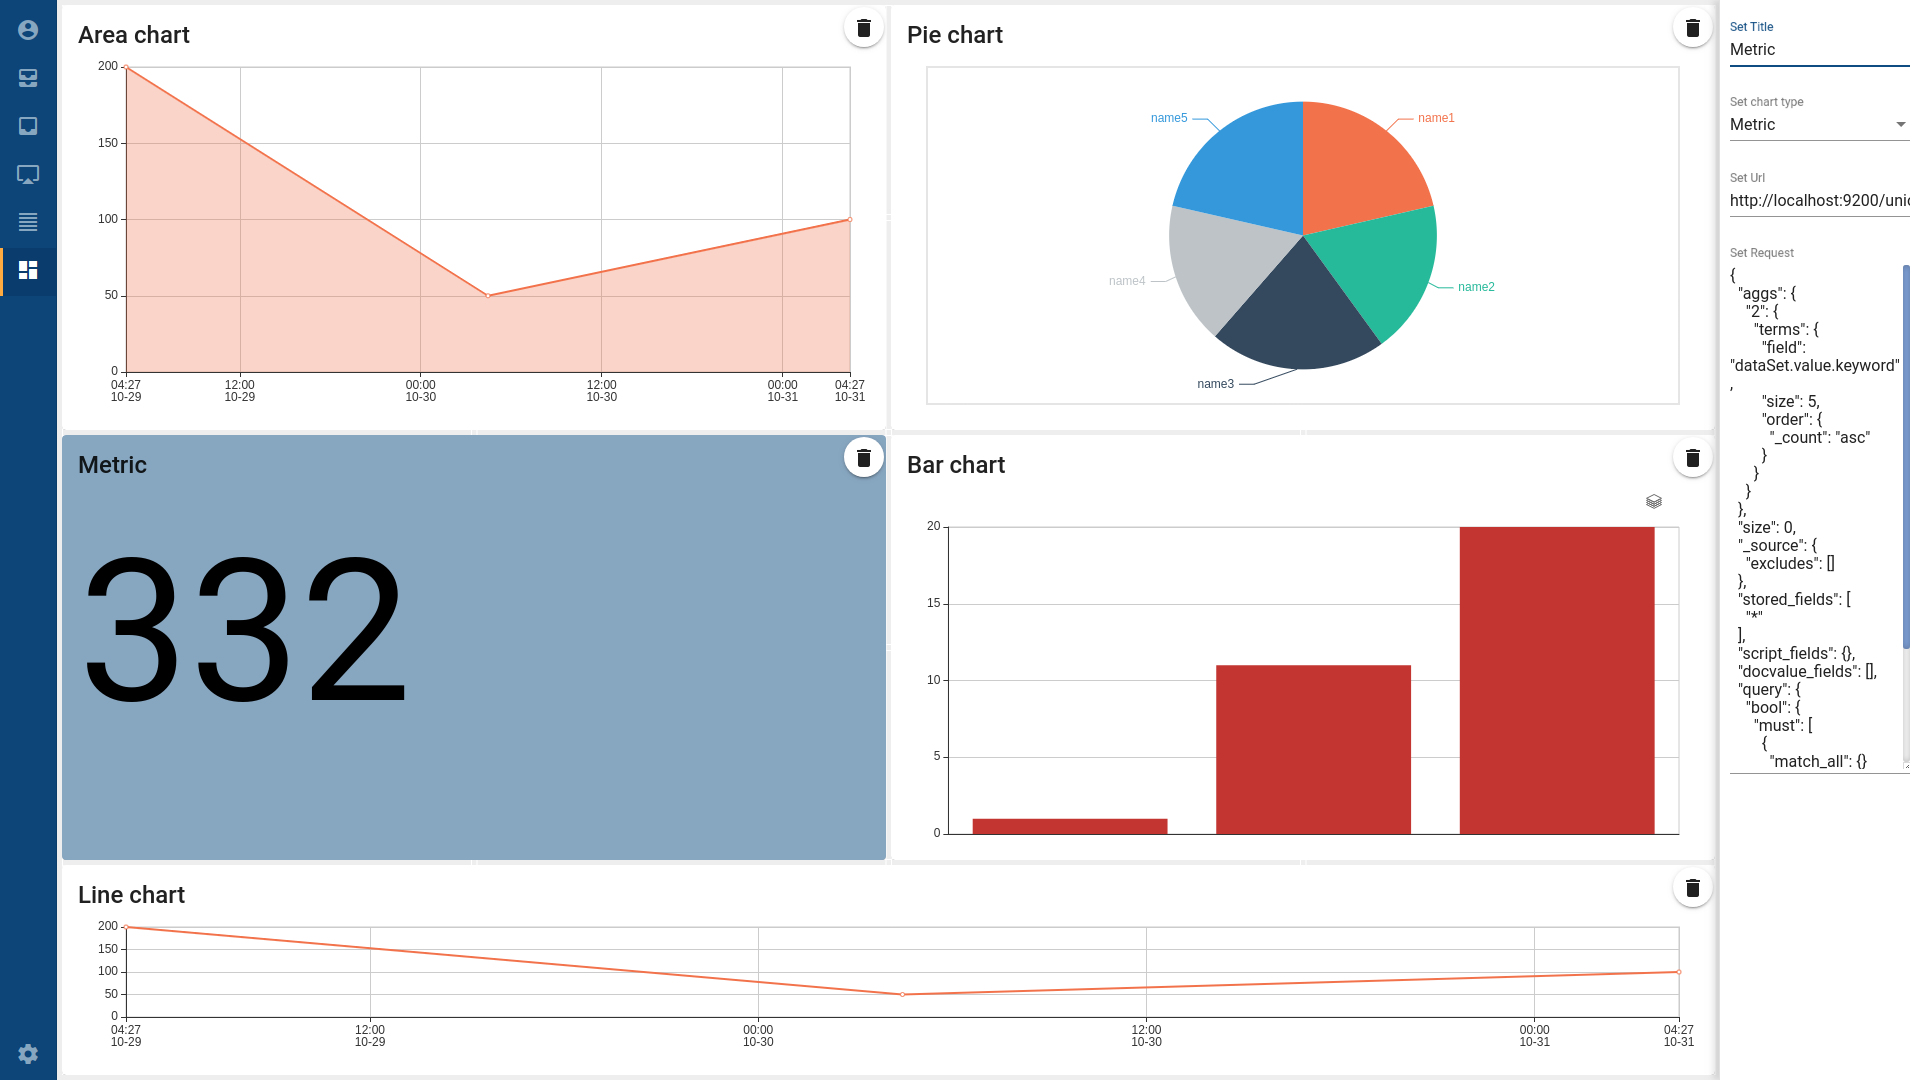
\includegraphics[width=0.9\textwidth]{images/dashboard_view.png}
  \caption{Dashboard view}
  \label{fig:dashboard}
\end{figure}

\subsection{Elasticsearch and Kibana}\label{subsec:elasticsearch-and-kibana}

Data for visualisation are loaded from an Elasticsearch instance running on the specified URL\@.
Elasticsearch query has to be specified in the request field.
You can use Kibana for creating the request.
Create a new visualisation in Kibana following the official tutorial on \url{https://www.elastic.co/guide/en/kibana/current/tutorial-visualizing.html}.
On the top toolbar click on the Inspect button.
This will open a side panel with more details about the visualisation including raw data, statistics, request, and response.
From the \texttt{View} dropdown menu on the right select \texttt{Request} and switch to the \texttt{Request} tab.
Finally, copy the request body into the request field of a dashboard visualisation in the \builder.
